In this chapter, we will examine a brief review of the project's functions and the system's scenarios and use cases. This section includes the entire functional specification.

\section{Overall System Requirements}
In general, this application should satisfy the following requirements:
\begin{itemize}
  \item A login system with authentication
  \item Users can upload and download files
  \item The system limited users with some features
  \begin{itemize}
    \item For Admin:
        \begin{itemize}
            \item Manage Users
            \item Manage User Groups
            \item Access to all files and folders
            \item Grant or remove permissions for all files and folders
        \end{itemize}
    \item For Regular Users:
        \begin{itemize}
            \item View their own profile
            \item Update their own profile
            \item Access to files and folders they have permission to read and/or write
            \item Grant or remove permissions for the files or folders they own
        \end{itemize}
  \end{itemize}
\end{itemize}

\section{Users \& Non-functional Requirements}
\begin{itemize}
    \item \textbf{Users Requirement}: Have a device with internet access, preferable Chrome web browser
    \item \textbf{Performance}: The website is accessible by anyone with a public domain. 
    \item \textbf{Availability}: The user can only work with the system fully if they can login with a registered account.
    \item \textbf{Re-usability}: User can use external files with the website. User can use CSV file generated from the website for other purposes. The data generated by the website can be use as the resource for other services.
    \item \textbf{Reliability}: The system will not work without the Internet connection.
\end{itemize}

\section{Use Cases}
\subsection{Use Cases Diagram}
The following diagram describes the functions that a user can perform with the system.
\begin{figure}[H]
    \centering
    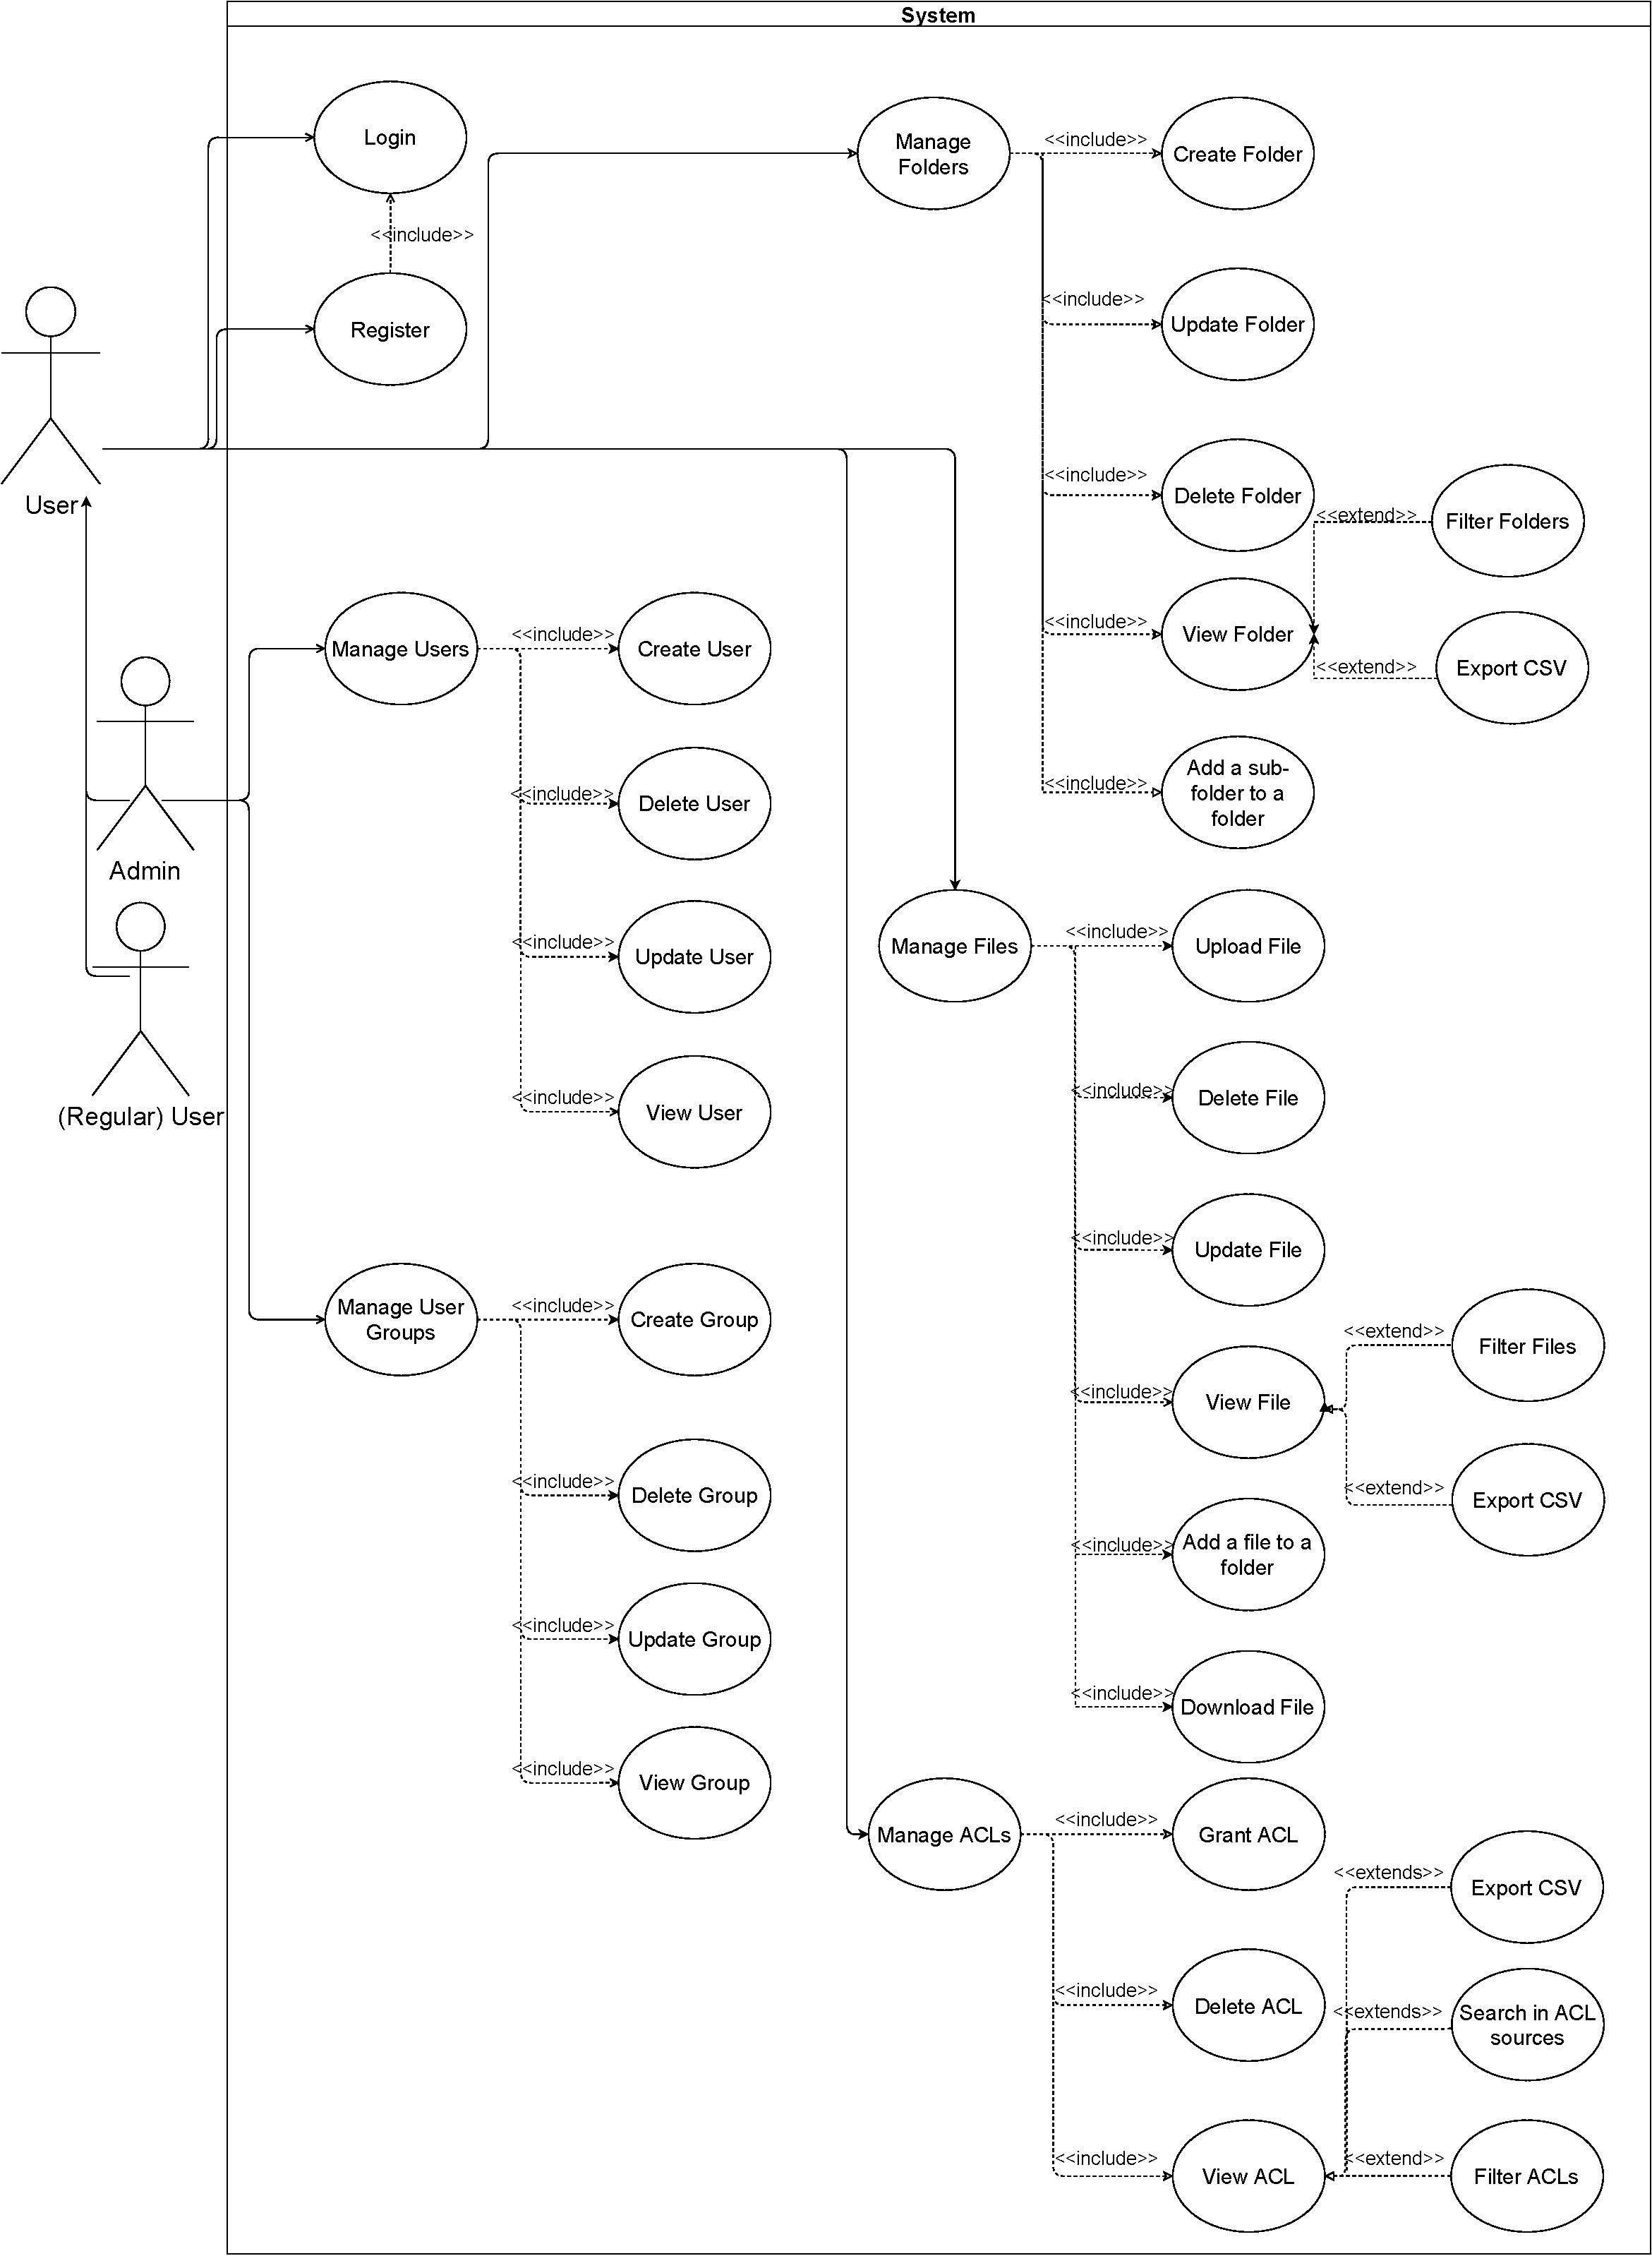
\includegraphics[width=0.95\textwidth]{images/Use_case_diagram_Top_level_All.pdf}
    \caption{Use cases diagram}
    \label{fig:description}
\end{figure}
\subsection{Users Characteristics}
Two types of users interact with the system: \textbf{Admin} and (regular) \textbf{User}. Each user type has different uses in the system, so each of them has its requirements:
\begin{itemize}
    \item \textbf{Admin}: a user who has access to all resources; only admin could manage user groups, total management of users
    \item \textbf{User}: a user who only has access to the resource they have permission to use, only could view and edit their profile.
\end{itemize}

\section{Use Case and Scenario Description}
\subsection{Use case: Register (SUB-FEATURE 1.1)}
\subsubsection{Brief description}
This use case describes how a user registers to the system. 
\subsubsection{Flow of events} 
\textbf{1. Basic Flow}

The table \ref{table:1} takes place when one person wants to create a new account on the system.
\begin{table}[H]
\centering
\begin{tabulary}{1.0\textwidth}{ |L|L|L| }
  \hline
    \rowcolor{gray} 
    \textbf{Actor Action} & 
    \textbf{System Action} & 
    \textbf{Data} \\
  \hline 
   & 1. The system requests that the Actor enter required information & - First name \newline- Last name \newline- Email \newline- Username \newline- Password \newline \\ 
  \hline
  2. The Actor enters their information. & 3. The system check the entered account exists on the system or not with username and email & \\
  \hline
  & 4. The system validates user’s information and create a new 
account for user and log the Actor into the system after created successfully & \\
  \hline 
\end{tabulary}
\caption{Register Basic Flow (SUB-FEATURE 1.1)}
\label{table:1}
\end{table}

\par
\textbf{2. Alternative Flows}

\begin{enumerate}[label=(\roman*)]
    \item Account exists \\
If in the Basic Flow, at step 3, the account has existed on the system, the system displays an error message. If the user goes back, return the form. The Actor can select to cancel the operation, at which point the Use Case ends.
    \item Invalid Format or Insufficient Information \\
If, in the Basic Flow, at step 2, the Actor has not specified sufficient information to create a new account as required, the system will prompt the Actor for the invalid field or the missing information. The Actor can either enter the missing information or cancel the operation, at which point the Use Case ends.
\end{enumerate}

\subsubsection{Special Requirement}
Only Regular Users can Register into the system. Admin is either pre-created or assigned an account. 
\subsubsection{Pre-conditions}
User is not logged in.
\subsubsection{Post-conditions}
If the use case is successful, the user registers successfully. If not, the system state is unchanged.

\subsection{Use case: Login (SUB-FEATURE 1.2)}
\subsubsection{Brief description}
The Use Case describes how a user logs into the system.
\subsubsection{Flow of events} 
\textbf{1. Basic Flow}
The table \ref{table:2} describe when the Actor wishes to Login to the system.
\begin{table}[H]
\centering
\begin{tabulary}{1.0\textwidth}{ |L|L|L| }
  \hline
    \rowcolor{gray} 
    \textbf{Actor Action} & 
    \textbf{System Action} & 
    \textbf{Data} \\
  \hline 
   & 1. The system requests that the Actor enter their username and password & - Username* \newline- Password* \newline* Required fields \\ 
  \hline
  2. The Actor enters their email and password. & 3. The system validates the entered name and password and logs the Actor into the system. & \\
  \hline 
\end{tabulary}
\caption{Login Basic Flow (SUB-FEATURE 1.2)}
\label{table:2}
\end{table}

\par
\textbf{2. Alternative Flows}

\begin{enumerate}[label=(\roman*)]
    \item Invalid Username/Password \\
If in the Basic Flow, at step 2, the Actor enters an invalid username or password, the system displays an error message. The Actor can either return to the beginning of the Basic Flow or cancel the login, at which point the Use Case ends.
\end{enumerate}

\subsubsection{Special Requirement}
None.
\subsubsection{Pre-conditions}
The user account must exist.
\subsubsection{Post-conditions}
If the Use Case was successful, the Actor is now logged into the system. If not, the system state is unchanged.

\subsection{Use case: Manage Users (FEATURE 2)}
\subsubsection{Brief description}
The Use Case allows the system Admin to manage users' information. This includes adding a new user to the system, changing existing users' information on the system, removing a user from the system, and viewing a user.
\subsubsection{Flow of events} 
\textbf{1. Basic Flow}
The table \ref{table:3} describe when the Admin wishes to add, change, and/or delete User information in the system.
\begin{table}[H]
\centering
\begin{tabulary}{1.0\textwidth}{ |L|L|L| }
  \hline
    \rowcolor{gray} 
    \textbf{Actor Action} & 
    \textbf{System Action} & 
    \textbf{Data} \\
   \hline 
  1. The Admin wants to manage users. & 2. The system shows list of all users. & List of all users details.\\
  \hline 
  3. The Admin views the users lists and/or filers them by custom criteria. & 4. The system displays the users by custom criteria. & List of all users with custom criteria.\\
  \hline
  & 5. The system requests that the Admin specifies  the function he/she would like to perform (either Create a User, Update User or Delete User). & - Manage selection \\ 
  \hline
  6. The Admin selects "Create User". & 7. The system requests the
Administrator to enter the User information. &  - Username* \newline- Password* \newline- Email* \newline- First Name \newline- Last Name \newline- Department \newline- Affiliation \newline* Required fields \\
  \hline 
  8. The Admin provides the requested information. & 9. The system generates and assigns a unique User Id number to the user. The User is added to the system.  & \\
  \hline 
\end{tabulary}
\caption{Manage Users Basic Flow (SUB-FEATURE 2.1 \& SUB-FEATURE 2.2)}
\label{table:3}
\end{table}

\emph{Update User Sub Flow} \par
At step 6 of \textbf{Basic Flow }
\begin{table}[H]
\centering
\begin{tabulary}{1.0\textwidth}{ |L|L|L| }
  \hline
    \rowcolor{gray} 
    \textbf{Actor Action} & 
    \textbf{System Action} & 
    \textbf{Data} \\
  \hline 
  1. The Admin selects "Update User". & 2. The system requests the Admin to select User from User list or User profile interface. & \\ 
  \hline
  3. The Admin selects User. & 4. The system retrieves and displays the User. &  \\
  \hline 
  5. The Admin enter the desired changes to the User information. & 6. The system updates the User record with the updated information. & \newline- First Name \newline- Last Name \newline- Department \newline- Affiliation \\
  \hline 
\end{tabulary}
\caption{Update User Sub Flow (SUB-FEATURE 2.3)}
\label{table:5}
\end{table}

\emph{Delete User Sub Flow} \par
At step 6 of \textbf{Basic Flow }
\begin{table}[H]
\centering
\begin{tabulary}{1.0\textwidth}{ |L|L|L| }
  \hline
    \rowcolor{gray} 
    \textbf{Actor Action} & 
    \textbf{System Action} & 
    \textbf{Data} \\
  \hline 
  1. The Admin selects "Delete User". & 2. The system requests the Admin to select User from User list or User profile interface. & \\ 
  \hline
  3. The Admin selects User. & 4. The system retrieves and displays the User. &  \\
  \hline 
  5. The Admin select delete. & 6. The system removes the User from the system.& \\
  \hline 
\end{tabulary}
\caption{Delete User Sub Flow (SUB-FEATURE 2.4)}
\label{table:4}
\end{table}

\par
\textbf{2. Alternative Flows}

\begin{enumerate}[label=(\roman*)]
    \item User not found \\
If in the Update User sub flow, at step 3 or Delete User sub flow, at step 3, a User with the specified id number does not exist, the system displays an error message. The Administrator can cancel the operation, at which point the Use Case ends.
\end{enumerate}

\subsubsection{Special Requirement}
None.
\subsubsection{Pre-conditions}
The Admin must be logged into the system before this Use Case begins.
\subsubsection{Post-conditions}
If the Use Case was successful, the User information is created, updated, deleted from the system. Otherwise, the system state is unchanged.

\subsection{Use case: Manage User Groups (FEATURE 3)}
\subsubsection{Brief description}
The Use Case allows the system Admin to manage user groups' information. This includes adding a new group to the system, changing existing group' information on the system, removing a group from the system, and viewing a group.
\subsubsection{Flow of events} 
\textbf{1. Basic Flow}
The table \ref{table:6} describe when the Admin wishes to add, change, and/or delete Group information in the system.
\begin{table}[H]
\centering
\begin{tabulary}{1.0\textwidth}{ |L|L|L| }
  \hline
    \rowcolor{gray} 
    \textbf{Actor Action} & 
    \textbf{System Action} & 
    \textbf{Data} \\
   \hline 
  1. The Admin wants to manage groups. & 2. The system shows list of all groups. & List of all groups details.\\
  \hline 
  3. The Admin views the groups lists and/or filter groups by custom criteria. & 4. The system displays the groups by custom criteria. & List of all groups with custom criteria.\\
  \hline
  & 5. The system requests that the Admin specify the function he/she would like to perform (either Create a Group, Update Group or Delete Group). & Manage selection \\ 
  \hline
  6. The Admin selects "Create Group". & 7. The system requests the
Administrator to enter the User information. & Name* \\
  \hline 
  8. The Admin provides the requested information. & 9. The system generates and assigns a unique Group Id number to the user. The Group is added to the system.  & \\
  \hline 
\end{tabulary}
\caption{Manage Groups Basic Flow (SUB-FEATURE 3.1 \& SUB-FEATURE 3.1)}
\label{table:6}
\end{table}

\emph{Update Group Sub Flow} \par
At step 6 of \textbf{Basic Flow }
\begin{table}[H]
\centering
\begin{tabulary}{1.0\textwidth}{ |L|L|L| }
  \hline
    \rowcolor{gray} 
    \textbf{Actor Action} & 
    \textbf{System Action} & 
    \textbf{Data} \\
  \hline 
  1. The Admin selects "Update Group". & 2. The system requests the Admin to select Group from Group list or Group details interface. & \\ 
  \hline
  3. The Admin selects Group. & 4. The system retrieves and displays the Group along with a list of all users. &  \\
  \hline 
  5. The Admin adds a user from User list to a group. & 6. The system updates the Group record with the updated information. &  Username  \\
  \hline 
\end{tabulary}
\caption{Update Group Sub Flow (SUB-FEATURE 3.3)}
\label{table:8}
\end{table}

\emph{Delete Group Sub Flow} \par
At step 6 of \textbf{Basic Flow }
\begin{table}[H]
\centering
\begin{tabulary}{1.0\textwidth}{ |L|L|L| }
  \hline
    \rowcolor{gray} 
    \textbf{Actor Action} & 
    \textbf{System Action} & 
    \textbf{Data} \\
  \hline 
  1. The Admin selects "Delete Group". & 2. The system requests the Admin to select Group from Group list or Group details interface. & \\ 
  \hline
  3. The Admin selects Group. & 4. The system retrieves and displays the Group. &  \\
  \hline 
  5. The Admin select delete. & 6. The system removes the Group from the system.& \\
  \hline 
\end{tabulary}
\caption{Delete Group Sub Flow (SUB-FEATURE 3.4)}
\label{table:7}
\end{table}
\par
\textbf{2. Alternative Flows}

\begin{enumerate}[label=(\roman*)]
    \item Group not found \\
If in the Update Group sub flow, at step 3 or Delete Group sub flow, at step 3, a Group with the specified id number does not exist, the system displays an error message. The Administrator can cancel the operation, at which point the Use Case ends.
\end{enumerate}

\subsubsection{Special Requirement}
None.
\subsubsection{Pre-conditions}
The Admin must be logged into the system before this Use Case begins.
\subsubsection{Post-conditions}
If the Use Case was successful, the Group information is created, updated, deleted from the system. Otherwise, the system state is unchanged.

\subsection{Use case: Manage Folders (FEATURE 4)}
\subsubsection{Brief description}
The Use Case allows the system users to manage folders' information. This includes adding a new folder to the system, changing existing folders' information on the system, removing a folder from the system, and viewing a folder.
\subsubsection{Flow of events} 
\textbf{1. Basic Flow}
The table \ref{table:9} describe when the users wish to add, change, and/or delete Folder information in the system.
\begin{table}[H]
\centering
\begin{tabulary}{1.0\textwidth}{ |L|L|L| }
  \hline
    \rowcolor{gray} 
    \textbf{Actor Action} & 
    \textbf{System Action} & 
    \textbf{Data} \\
   \hline 
  1. The users want to manage folders. & 2. The system shows the list of all folders and files details. & \\
  \hline 
  3. The users view the folders and files lists and/or filter them by custom criteria. & 4. The system displays the files and folders by custom criteria. & List of all files and folders with custom criteria.\\
  \hline
  & 5. The system requests that the users specify the function he/she would like to perform (either Create a Folder, Update Folder, Move Folder, or Delete Folder). & - Manage selection \\ 
  \hline
  6. The users select "Create Folder". & 7. The system requests the
users to enter the Folder information. &  - Name* \newline- Source* \newline- Topics* \newline* Required fields \\
  \hline 
  8. The users provide the requested information. & 9. The system generates and assigns a unique Folder Id number to the User. The Folder is added to the system.  The User is recognized as the Folder's owner by the system with read and write permission. Permission for Admin is also automatically added. & \\
  \hline 
\end{tabulary}
\caption{Manage Folders Basic Flow (SUB-FEATURE 4.1 \&  SUB-FEATURE 4.2)}
\label{table:9}
\end{table}

\emph{Edit Folder Sub Flow} \par
At step 6 of \textbf{Basic Flow }
\begin{table}[H]
\centering
\begin{tabulary}{1.0\textwidth}{ |L|L|L| }
  \hline
    \rowcolor{gray} 
    \textbf{Actor Action} & 
    \textbf{System Action} & 
    \textbf{Data} \\
  \hline 
  1. The users select "Update Folder". & 2. The system requests the users to select Folder from Folder list or Folder details interface. & \\ 
  \hline
  3. The users select Folder. & 4. The system retrieves and displays the Folder. &  \\
  \hline 
  5. The users enter the desired changes to the Folder information. & 6. The system updates the Folder record with the updated information. & \newline- Name \newline- Source \newline- Topics \\
  \hline 
\end{tabulary}
\caption{Edit Folder Sub Flow (SUB-FEATURE 4.3)}
\label{table:11}
\end{table}
\par

\emph{Move a Sub-folder to a Folder Sub Flow} \par
At step 6 of \textbf{Basic Flow}
\begin{table}[H]
\centering
\begin{tabulary}{1.0\textwidth}{ |L|L|L| }
  \hline
    \rowcolor{gray} 
    \textbf{Actor Action} & 
    \textbf{System Action} & 
    \textbf{Data} \\
  \hline 
1. The users select "Move Folder". & 2. The system requests the users to select Folder from Folder list or Folder details interface. & \\ 
  \hline
3. The users select Folder. & 4. The system retrieves and displays the Folder. &  \\
  \hline 
5. The users enter the destination folder name. & 6. The system updates the Folder record with the updated information. & Destination Folder name \\
  \hline 
\end{tabulary}
\caption{Move a sub-folder to a Folder Sub Flow (SUB-FEATURE 4.4)}
\label{table:12}
\end{table}
\par

\emph{Delete Folder Sub Flow} \par
At step 6 of \textbf{Basic Flow }
\begin{table}[H]
\centering
\begin{tabulary}{1.0\textwidth}{ |L|L|L| }
  \hline
    \rowcolor{gray} 
    \textbf{Actor Action} & 
    \textbf{System Action} & 
    \textbf{Data} \\
  \hline 
  1. The users selects "Delete Folder". & 2. The system requests the users to select Folder from Folder list or Folder details interface. & \\ 
  \hline
  3. The users selects Folder. & 4. The system retrieves and displays the Folder. &  \\
  \hline 
  5. The users select delete. & 6. The system removes the Folder from the system.& \\
  \hline 
\end{tabulary}
\caption{Delete Folder Sub Flow (SUB-FEATURE 4.5)}
\label{table:10}
\end{table}
\par

\textbf{2. Alternative Flows}

\begin{enumerate}[label=(\roman*)]
    \item Folder not found \\
If in the Update Folder sub flow, at step 3 or Delete Folder sub flow, at step 3, a Folder with the specified id number does not exist, the system displays an error message. The users can cancel the operation, at which point the Use Case ends.
    \item Invalid Format or Insufficient Information\\
If, in the Create Folder sub flow, at step 7; in the Edit Folder and Move Folder sub flow, at step 5, the users have not specified sufficient information to add a new Folder, the system will prompt the users for the missing information. The users can either enter the missing information or choose to cancel the operation, at which point the Use Case ends.
    \item The users do not have the permission to view\\
If, in the Basic Flow at step 2, the users do not have the right to view a folder. The folder doesn't appear in the list of all files and folders.
    \item The users do not have the permission to write\\
If, in the Edit Folder, Move Folder and Delete Folder sub flow, at step 5, the users do not have the right to write folder. The users can choose to cancel the operation, at which point the Use Case ends.
\end{enumerate}

\subsubsection{Special Requirement}
None.
\subsubsection{Pre-conditions}
The users must be logged into the system before this Use Case begins.
\subsubsection{Post-conditions}
If the Use Case was successful, the Folder information is created, updated, deleted from the system. Otherwise, the system state is unchanged.

\subsection{Use case: Manage Files (FEATURE 5)}
\subsubsection{Brief description}
The Use Case allows the system users to manage files' information. This includes upload a new file to the system, changing existing files' information on the system, removing a file from the system, and viewing a file.
\subsubsection{Flow of events} 
\textbf{1. Basic Flow}
The table \ref{table:13} describe when the users wish to upload, change, and/or delete File information in the system.
\begin{table}[H]
\centering
\begin{tabulary}{1.0\textwidth}{ |L|L|L| }
  \hline
    \rowcolor{gray} 
    \textbf{Actor Action} & 
    \textbf{System Action} & 
    \textbf{Data} \\
   \hline 
  1. The users want to manage files. & 2. The system shows the list of all folders and files details. &\\
  \hline 
  3. The users view the folders and files lists and/or filter them by custom criteria. & 4. The system displays the files and folders by custom criteria. & List of all files and folders with custom criteria.\\
  \hline
  & 5. The system requests that the users specify the function he/she would like to perform (either Create a File, Update File, Move File, Download File, or Delete File). & - Manage selection \\ 
  \hline
  6. The users select "Upload File". & 7. The system requests the
users to enter the File information. &  - File(s) Data* \newline- Source* \newline- Topics* \newline* Required fields \\
  \hline 
  8. The users provide the requested information. & 9. The system generates and assigns a unique File Id number to the User. The File is uploaded to the system.  The User is recognized as the File's owner by the system with read and write permission. Permission for Admin is also automatically uploaded. & \\
  \hline 
\end{tabulary}
\caption{Manage Files Basic Flow (SUB-FEATURE 5.1 \& SUB-FEATURE 5.2)} 
\label{table:13}
\end{table}

\emph{Edit File Sub Flow} \par
At step 6 of \textbf{Basic Flow }
\begin{table}[H]
\centering
\begin{tabulary}{1.0\textwidth}{ |L|L|L| }
  \hline
    \rowcolor{gray} 
    \textbf{Actor Action} & 
    \textbf{System Action} & 
    \textbf{Data} \\
  \hline 
  1. The users select "Update File". & 2. The system requests the users to select File from File list or File details interface. & \\ 
  \hline
  3. The users select File. & 4. The system retrieves and displays the File. &  \\
  \hline 
  5. The users enter the desired changes to the File information. & 6. The system updates the File record with the updated information. & \newline- Name \newline- Source \newline- Topics \\
  \hline 
\end{tabulary}
\caption{Update File Sub Flow (SUB-FEATURE 5.3)}
\label{table:15}
\end{table}
\par

\emph{Add a File to a Folder Sub Flow} \par
At step 6 of \textbf{Basic Flow }
\begin{table}[H]
\centering
\begin{tabulary}{1.0\textwidth}{ |L|L|L| }
  \hline
    \rowcolor{gray} 
    \textbf{Actor Action} & 
    \textbf{System Action} & 
    \textbf{Data} \\
  \hline 
1. The users select "Move File". & 2. The system requests the users to select File from File list or File details interface. & \\ 
  \hline
3. The users select File. & 4. The system retrieves and displays the File. &  \\
  \hline 
5. The users enter the destination folder name. & 6. The system updates the File record with the updated information. & Destination File name \\
  \hline 
\end{tabulary}
\caption{Add a File to a Folder Sub Flow (SUB-FEATURE 5.4)}
\label{table:16}
\end{table}
\par

\emph{Download File Sub Flow} \par
At step 6 of \textbf{Basic Flow }
\begin{table}[H]
\centering
\begin{tabulary}{1.0\textwidth}{ |L|L|L| }
  \hline
    \rowcolor{gray} 
    \textbf{Actor Action} & 
    \textbf{System Action} & 
    \textbf{Data} \\
  \hline 
1. The users select "Download File". & 2. The system requests the users to select File from files and folders list or File details interface. & \\ 
  \hline
3. The users select File. & 4. The system retrieves and displays the File. &  \\
  \hline 
5. The users select to download File. & 6. The system return the File data. & File Data \\
  \hline 
\end{tabulary}
\caption{Download File Sub Flow (SUB-FEATURE 5.5)}
\label{table:17}
\end{table}
\par

\emph{Delete File Sub Flow} \par
At step 6 of \textbf{Basic Flow }
\begin{table}[H]
\centering
\begin{tabulary}{1.0\textwidth}{ |L|L|L| }
  \hline
    \rowcolor{gray} 
    \textbf{Actor Action} & 
    \textbf{System Action} & 
    \textbf{Data} \\
  \hline 
  1. The users selects "Delete File". & 2. The system requests the users to select File from File list or File details interface. & \\ 
  \hline
  3. The users selects File. & 4. The system retrieves and displays the File. &  \\
  \hline 
  5. The users select delete. & 6. The system removes the File from the system.& \\
  \hline 
\end{tabulary}
\caption{Delete File Sub Flow (SUB-FEATURE 5.6)}
\label{table:14}
\end{table}
\par
\textbf{2. Alternative Flows}

\begin{enumerate}[label=(\roman*)]
    \item File not found \\
If in the Update File sub flow, at step 3 or Delete File sub flow, at step 3, a File with the specified id number does not exist, the system displays an error message. The users can cancel the operation, at which point the Use Case ends.
    \item Invalid Format or Insufficient Information\\
If, in the Upload File sub flow, at step 7; in the Edit File and Move File sub flow, at step 5, the users have not specified sufficient information to upload new File, the system will prompt the users for the missing information. The users can either enter the missing information or choose to cancel the operation, at which point the Use Case ends.
    \item The users do not have the permission to view\\
If, in the Basic Flow at step 2, and in the Download File sub flow at step 5, the users do not have the right to view a file. The file doesn't appear in the list of all files and folders. And the users can't download the file. 
    \item The users do not have the permission to write\\
If, in the Edit File, Move a File to a Folder and Delete File sub flow, at step 5, the users do not have the right to write folder. The users can choose to cancel the operation, at which point the Use Case ends.
\end{enumerate}

\subsubsection{Special Requirement}
None.
\subsubsection{Pre-conditions}
The users must be logged into the system before this Use Case begins.
\subsubsection{Post-conditions}
If the Use Case was successful, the File information is created, updated, deleted from the system. Otherwise, the system state is unchanged.

\subsection{Use case: Manage ACLs (FEATURE 6)}
\subsubsection{Brief description}
The Use Case allows the system users to manage ACLs' information. This includes adding a new ACL to the system, changing existing ACLs' information on the system, removing a ACL from the system, and viewing a ACL.
\subsubsection{Flow of events} 
\textbf{1. Basic Flow}
The table \ref{table:18} describe when the users wish to add, change, and/or delete ACL information in the system.
\begin{table}[H]
\centering
\begin{tabulary}{1.0\textwidth}{ |L|L|L| }
  \hline
    \rowcolor{gray} 
    \textbf{Actor Action} & 
    \textbf{System Action} & 
    \textbf{Data} \\
   \hline 
  1. The users want to manage ACLs. & 2. The system shows the list of all ACLs details of the selected file or folder. & \\
  \hline
  & 3. The system requests that the users specify the function he/she would like to perform (either Grant a ACL, or Delete ACL). & - Manage selection \\ 
  \hline
  4. The users select "Grant ACL". & 5. The system requests the users to enter the ACL information. &  - Source Name* \newline- Target Id* \newline- Source Type (File or Folder)* \newline- Target Type (User or Group)* \newline- Permission (Read or Write)* \newline* Required fields \\
  \hline 
  6. The users provide the requested information. & 7. The system generates and assigns a ACL permission to the source. The ACL permission is added to the system.  &  \\
  \hline
\end{tabulary}
\caption{Manage ACLs Basic Flow (SUB-FEATURE 6.1 \& SUB-FEATURE 6.2)}
\label{table:18}
\end{table}

\emph{Delete ACL Sub Flow} \par
At step 3 of \textbf{Basic Flow }
\begin{table}[H]
\centering
\begin{tabulary}{1.0\textwidth}{ |L|L|L| }
  \hline
    \rowcolor{gray} 
    \textbf{Actor Action} & 
    \textbf{System Action} & 
    \textbf{Data} \\
  \hline 
  1. The users selects "Delete ACL". & 2. The system requests the users to select ACL from ACL list. & \\ 
  \hline
  3. The users select delete. & 4. The system removes the ACL from the system.& \\
  \hline 
\end{tabulary}
\caption{Delete ACL Sub Flow (SUB-FEATURE 6.3)}
\label{table:19}
\end{table}
\textbf{2. Alternative Flows}

\begin{enumerate}[label=(\roman*)]
    \item ACL not found \\
If in Delete ACL sub flow, at step 3, a ACL with the specified id number does not exist, the system displays an error message. The users can cancel the operation, at which point the Use Case ends.
    \item The users do not have the permission to view\\
If, in the Basic Flow at step 2, the users do not have the right to view a file or a folder. They can not know the file or folder permission details. 
    \item The users do not have the permission to write\\
If, in the Delete sub flow, at step 2, the users do not have the right to write the selected file or folder. The users can choose to cancel the operation, at which point the Use Case ends.
    \item Invalid Format or Insufficient Information\\
If, in the Grant ACL sub flow, at step 5; the users have not specified sufficient information to add a new ACL, the system will prompt the users for the missing information. The users can either enter the missing information or choose to cancel the operation, at which point the Use Case ends.
\end{enumerate}

\subsubsection{Special Requirement}
None.
\subsubsection{Pre-conditions}
The users must be logged into the system before this Use Case begins.
\subsubsection{Post-conditions}
If the Use Case was successful, the ACL information is created or deleted from the system. Otherwise, the system state is unchanged.
